\documentclass{article}

% content/resources/templates/preamble.tex
\usepackage[margin=0.6in]{geometry}
\author{Milav Dabgar}
\usepackage{amsmath,amssymb,amsthm}
\usepackage{booktabs}
\usepackage{multirow}
\usepackage{xcolor}
\usepackage{tcolorbox}
\tcbuselibrary{breakable,skins}
\usepackage[colorlinks=true,linkcolor=blue]{hyperref}
\usepackage{titlesec}
\usepackage{enumitem}
\usepackage{tikz}
\usepackage{pgfplots}
\usepackage{circuitikz}
\usepackage[version=4]{mhchem}
\usepackage{longtable}
\usepackage{array}
\usepackage{float}
\usepackage{caption}
\usepackage{listings}

\lstset{
  basicstyle=\small\ttfamily,
  breaklines=true,
  breakatwhitespace=false,
  postbreak=\mbox{\textcolor{red}{$\hookrightarrow$}\space},
  float=false,
  numbers=left,
  numberstyle=\tiny\color{gray},
  numbersep=10pt,
  xleftmargin=2em,
  keywordstyle=\color{blue},
  commentstyle=\color{green!60!black},
  stringstyle=\color{purple},
  backgroundcolor=\color{gray!5},
  showstringspaces=false,
  tabsize=2,
  captionpos=b,
  keepspaces=true,
  columns=flexible
}

\pgfplotsset{compat=1.18}
\usetikzlibrary{shapes,arrows,positioning,calc,patterns,decorations.pathmorphing,decorations.markings,arrows.meta}

% Color scheme
\definecolor{headcolor}{RGB}{0,102,204}
\definecolor{keycolor}{RGB}{220,20,60}
\definecolor{solutioncolor}{RGB}{34,139,34}
\definecolor{mnemoniccolor}{RGB}{148,0,211}
\definecolor{codecolor}{RGB}{0,0,100}

% Spacing
\setlength{\parskip}{3pt}
\setlist[itemize]{nosep}
\setlist[enumerate]{nosep}

% Title formatting
\titleformat{\section}{\Large\bfseries\color{headcolor}}{\thesection}{1em}{}
\titleformat{\subsection}{\large\bfseries\color{headcolor}}{\thesubsection}{1em}{}

% Pandoc tightlist compatibility
\providecommand{\tightlist}{%
  \setlength{\itemsep}{0pt}\setlength{\parskip}{0pt}}

% Pandoc longtable compatibility
\newcounter{none}
\def\thenone{}


% content/resources/templates/english-boxes.tex

% Custom environments
\newtcolorbox{solutionbox}{
 breakable,
 enhanced,
 colback=solutioncolor!5!white,
 colframe=solutioncolor!75!black,
 fonttitle=\bfseries,
 title=Solution
}

\newtcolorbox{solutionboxnobreak}{
 colback=solutioncolor!5!white,
 colframe=solutioncolor!75!black,
 fonttitle=\bfseries,
 title=Solution
}

\newtcolorbox{keyformula}{
 breakable,
 enhanced,
 colback=keycolor!5!white,
 colframe=keycolor!75!black,
 fonttitle=\bfseries,
 title=Key Formula
}

\newtcolorbox{mnemonicboxenv}{
 breakable,
 enhanced,
 colback=mnemoniccolor!5!white,
 colframe=mnemoniccolor!75!black,
 fonttitle=\bfseries,
 title=Mnemonic
}

\newcommand{\mnemonicbox}[1]{%
  \begin{mnemonicboxenv}
    #1
  \end{mnemonicboxenv}
}


% Custom commands for GTU solutions
% This file defines semantic commands for consistent formatting

% Question command with automatic formatting
\newcommand{\question}[2]{%
  \section*{Question #1}%
  \textbf{#2}%
}

% OR question variant
\newcommand{\questionor}[2]{%
  \section*{Question #1 OR}%
  \textbf{#2}%
}

% Proper table environment with caption
\newenvironment{answertable}[1]{%
  \begin{table}[htbp]
  \centering
  \caption{#1}
}{%
  \end{table}
}

% Proper figure environment for diagrams
\newenvironment{answerdiagram}[1]{%
  \begin{figure}[htbp]
  \centering
  \caption{#1}
}{%
  \end{figure}
}

% Semantic markup for key terms
\newcommand{\keyword}[1]{\textbf{#1}}
\newcommand{\code}[1]{\texttt{#1}}
\newcommand{\classname}[1]{\texttt{#1}}
\newcommand{\methodname}[1]{\texttt{#1}}

% Proper quotation marks
\newcommand{\mnemonic}[1]{``#1''}


\title{Microprocessor \& Microcontroller Systems (1333202) - Summer 2024 Solution}
\date{June 10, 2024}

\begin{document}
\maketitle

\questionmarks{1(a)}{3}{List common features of 8051 microcontroller.}

\begin{solutionbox}
The 8051 is a popular 8-bit microcontroller with the following key features:

\begin{center}
\captionof{table}{Common Features of 8051}
\begin{tabulary}{\linewidth}{|L|L|}
\hline
\textbf{Feature} & \textbf{Description} \\ \hline
\textbf{On-chip Oscillator} & Built-in clock generator circuit (typically 12MHz) \\ \hline
\textbf{Program Memory} & 4KB internal ROM for code storage \\ \hline
\textbf{Data Memory} & 128 bytes internal RAM for variables \\ \hline
\textbf{I/O Ports} & 4 bidirectional 8-bit ports (P0, P1, P2, P3) \\ \hline
\textbf{Timers/Counters} & Two 16-bit Timer/Counter units (Timer 0, Timer 1) \\ \hline
\textbf{Serial Port} & One Full duplex UART channel for communication \\ \hline
\textbf{Interrupts} & 5 interrupt sources (2 external, 2 timer, 1 serial) with priority levels \\ \hline
\textbf{SFRs} & Special Function Registers for system control \\ \hline
\end{tabulary}
\end{center}
\end{solutionbox}

\begin{mnemonicbox}
\mnemonic{On Program Data I/O Timers Serial Interrupts SFRs}
\end{mnemonicbox}

\questionmarks{1(b)}{4}{Define T-State, Machine Cycle, Instruction Cycle and Opcode.}

\begin{solutionbox}
These terms define the timing and operation of a microprocessor:

\begin{center}
\captionof{table}{Microprocessor Timing Definitions}
\begin{tabulary}{\linewidth}{|L|L|L|}
\hline
\textbf{Term} & \textbf{Definition} & \textbf{Duration/Size} \\ \hline
\textbf{T-State} & One subdivision of the operation performed in one clock period. It is the basic unit of time. & $1/f_{clk}$ \\ \hline
\textbf{Machine Cycle} & Time required to complete one memory access (read/write) or I/O operation. & 3-6 T-states (8085) \\ \hline
\textbf{Instruction Cycle} & Time required to fetch, decode, and execute a complete instruction. & 1-5 Machine cycles \\ \hline
\textbf{Opcode} & Operation Code: The part of the instruction that specifies the operation to be performed. & 1 byte \\ \hline
\end{tabulary}
\end{center}

\begin{itemize}
    \item \keyword{T-State}: Smallest unit of processing time.
    \item \keyword{Machine Cycle}: Basic CPU operation (Fetch, Read, Write).
    \item \keyword{Instruction Cycle}: Cycle = Fetch + Decode + Execute.
\end{itemize}
\end{solutionbox}

\begin{mnemonicbox}
\mnemonic{Time Machine Instruction Operation}
\end{mnemonicbox}

\questionmarks{1(c)}{7}{Compare Von-Neumann and Harvard Architecture.}

\begin{solutionbox}
Here is the comparison between the two major computer architectures:

\begin{center}
\captionof{table}{Von-Neumann vs Harvard Architecture}
\begin{tabulary}{\linewidth}{|L|L|L|}
\hline
\textbf{Parameter} & \textbf{Von-Neumann} & \textbf{Harvard} \\ \hline
\textbf{Memory Organization} & Single shared memory for both Code and Data. & Separate physical memory for Program Code and Data. \\ \hline
\textbf{Bus Structure} & Single bus for fetching instruction and data. & Separate buses for instruction and data. \\ \hline
\textbf{Speed} & Slower execution due to serial fetching (bottleneck). & Faster execution as instruction and data can be fetched simultaneously. \\ \hline
\textbf{Cost} & Simpler hardware, lower cost. & More buses, bigger control unit, higher cost. \\ \hline
\textbf{Flexibility} & Efficient use of memory (code/data boundary is flexible). & Fixed amount of memory for code and data. \\ \hline
\textbf{Examples} & 8085, x86 PCs. & 8051, DSP chips. \\ \hline
\end{tabulary}
\end{center}

\begin{center}
\begin{tikzpicture}[node distance=1.5cm]
    % Von Neumann
    \node [gtu block, minimum width=3cm] (cpu1) {CPU};
    \node [gtu block, minimum width=3cm, below=2cm of cpu1] (mem1) {Memory\\(Code + Data)};
    \draw [gtu arrow, <->] (cpu1) -- node[right, font=\small] {Single Bus} (mem1);
    \node [above=0.2cm of cpu1, font=\bfseries] {Von-Neumann};

    % Harvard
    \node [gtu block, minimum width=3cm, right=4cm of cpu1] (cpu2) {CPU};
    \node [gtu block, below right=2cm of cpu2] (dmem) {Data\\Memory};
    \node [gtu block, below left=2cm of cpu2] (pmem) {Program\\Memory};
    \draw [gtu arrow, <->] (cpu2) -- node[right, font=\small, pos=0.4] {Data Bus} (dmem);
    \draw [gtu arrow, <->] (cpu2) -- node[left, font=\small, pos=0.4] {Code Bus} (pmem);
    \node [above=0.2cm of cpu2, font=\bfseries] {Harvard};
\end{tikzpicture}
\captionof{figure}{Architecture Comparison}
\end{center}
\end{solutionbox}

\begin{mnemonicbox}
\mnemonic{Von-Single Harvard-Dual}
\end{mnemonicbox}

\questionmarks{1(c) OR}{7}{Explain Microcomputer System with block diagram.}

\begin{solutionbox}
A microcomputer system consists of a CPU, memory, I/O devices, and a system bus interconnecting them.

\begin{center}
\begin{tikzpicture}[node distance=1.5cm]
    \node [gtu block, minimum width=3cm, minimum height=2cm] (cpu) {CPU\\(MPU)};
    \node [gtu block, right=1cm of cpu, minimum height=2cm] (mem) {Memory\\(ROM/RAM)};
    \node [gtu block, right=1cm of mem, minimum height=2cm] (io) {I/O Devices\\(Peripherals)};
    
    % Buses
    \draw [gtu arrow, <->] (cpu) -- node[below] {System Bus} (mem);
    \draw [gtu arrow, <->] (mem) -- (io);
    
    % Detailed bus representation
    \coordinate (bus_start) at ($(cpu.south west) + (0,-1)$);
    \coordinate (bus_end) at ($(io.south east) + (0,-1)$);
    
    \draw [ultra thick] (bus_start) -- (bus_end) node[below left] {System Bus (Address, Data, Control)};
    
    \draw [<->, thick] (cpu.south) -- (cpu.south |- bus_start);
    \draw [<->, thick] (mem.south) -- (mem.south |- bus_start);
    \draw [<->, thick] (io.south) -- (io.south |- bus_start);
    
\end{tikzpicture}
\captionof{figure}{Microcomputer System Block Diagram}
\end{center}

\begin{center}
\captionof{table}{System Components}
\begin{tabulary}{\linewidth}{|L|L|L|}
\hline
\textbf{Component} & \textbf{Function} & \textbf{Example} \\ \hline
\textbf{CPU} & The "Brain". Fetches and executes instructions, reads/writes data. Control center. & 8085, 8086 \\ \hline
\textbf{Memory} & Stores instructions (ROM) and temporary data/variables (RAM). & EPROM, SRAM \\ \hline
\textbf{I/O Unit} & Interface to the outside world (Keyboard, Display, Sensors). & 8255 PPI \\ \hline
\textbf{System Bus} & Set of wires to transfer Information. Includes Address, Data, and Control buses. & Ribbon Cable \\ \hline
\end{tabulary}
\end{center}
\end{solutionbox}

\questionmarks{2(a)}{3}{Draw Bus organization in 8085 Microprocessor.}

\begin{solutionbox}
The 8085 has three sets of buses:

\begin{center}
\begin{tikzpicture}[node distance=2cm]
    \node [gtu block, minimum width=3cm, minimum height=2cm] (mp) {8085 CPU};
    
    \coordinate (busref) at ($(mp.east) + (1,0)$);
    
    % Address Bus
    \draw [gtu arrow, ->] ($(mp.east) + (0, 0.5)$) -- ++(2,0) node[right] {Address Bus (16-bit) [Unidirectional]};
    
    % Data Bus
    \draw [gtu arrow, <->] (mp.east) -- ++(2,0) node[right] {Data Bus (8-bit) [Bidirectional]};
    
    % Control Bus
    \draw [gtu arrow, ->] ($(mp.east) + (0, -0.5)$) -- ++(2,0) node[right] {Control Bus (Various) [Output/Input]};
    
    \node [right=0.5cm of mp.north east] {To Memory \& I/O};
\end{tikzpicture}
\captionof{figure}{8085 Bus Organization}
\end{center}
\end{solutionbox}

\questionmarks{2(b)}{4}{List Flags used in 8085 and Explain working of each flags.}

\begin{solutionbox}
The 8085 has a 5-bit Flag Register containing status flags that are set/reset by ALU operations.

\begin{center}
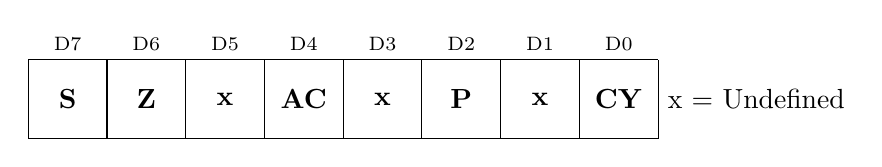
\begin{tikzpicture}
    % Flag Register
    \draw (0,0) grid (8,1);
    \foreach \x/\label in {0.5/D7, 1.5/D6, 2.5/D5, 3.5/D4, 4.5/D3, 5.5/D2, 6.5/D1, 7.5/D0}
        \node [above] at (\x, 1) {\scriptsize \label};
        
    \foreach \x/\val in {0.5/S, 1.5/Z, 2.5/x, 3.5/AC, 4.5/x, 5.5/P, 6.5/x, 7.5/CY}
        \node at (\x, 0.5) {\textbf{\val}};
        
    \node [right] at (8,0.5) {x = Undefined};
\end{tikzpicture}
\captionof{figure}{Flag Register Format}
\end{center}

\begin{center}
\captionof{table}{8085 Flags}
\begin{tabulary}{\linewidth}{|L|L|L|}
\hline
\textbf{Flag} & \textbf{Bit} & \textbf{Function} \\ \hline
\textbf{S (Sign)} & D7 & Set to 1 if MSB of result is 1 (Negative), else 0. \\ \hline
\textbf{Z (Zero)} & D6 & Set to 1 if result is Zero, else 0. \\ \hline
\textbf{AC (Aux Carry)} & D4 & Set to 1 if carry generated from D3 to D4 (Lower nibble to Upper nibble). Used in BCD. \\ \hline
\textbf{P (Parity)} & D2 & Set to 1 if result has even number of 1s (Even Parity), else 0. \\ \hline
\textbf{CY (Carry)} & D0 & Set to 1 if operation generates a carry/borrow out of MSB. \\ \hline
\end{tabulary}
\end{center}
\end{solutionbox}

\questionmarks{2(c)}{7}{Draw and Explain Block Diagram of 8085.}

\begin{solutionbox}
The 8085 architecture consists of the ALU, Timing \& Control Unit, Registers, and Interrupt control.

\begin{center}
\begin{tikzpicture}[scale=0.8, transform shape]
    % Main Blocks
    \node [gtu block] (alu) {ALU (8-bit)};
    \node [gtu block, below=1cm of alu] (acc) {Accumulator (A)};
    \node [gtu block, below=0.5cm of acc] (temp) {Temp Reg};
    \node [gtu block, right=1cm of acc] (flags) {Flags};
    
    \node [gtu block, right=3cm of alu, minimum width=3cm] (regs) {Register Array\\B, C, D, E, H, L\\SP, PC};
    
    \node [gtu block, left=2cm of acc] (id) {Instruction\\Decoder};
    \node [gtu block, below=1cm of id] (timing) {Timing \&\\Control Unit};
    
    \node [gtu block, above=1cm of regs] (interrupt) {Interrupt Control};
    \node [gtu block, above=1cm of alu] (serial) {Serial I/O Control};
    
    % Connections
    \draw [gtu arrow, <->] (alu) -- (acc);
    \draw [gtu arrow] (alu) -- (flags);
    \draw [gtu arrow] (id) -- (timing);
    \draw [gtu arrow, <->] (alu) -- (regs);
    
    % Buses
    \draw [->, thick] (regs.east) -- ++(1,0) node[right] {Address/Data Bus};
    \draw [->, thick] (timing.south) -- ++(0,-1) node[below] {Control Signals};
    
\end{tikzpicture}
\captionof{figure}{8085 Architecture Block Diagram}
\end{center}

\begin{center}
\captionof{table}{Functional Blocks}
\begin{tabulary}{\linewidth}{|L|L|}
\hline
\textbf{Block} & \textbf{Function} \\ \hline
\textbf{ALU} & Performs arithmetic (+, -) and logical (AND, OR) operations. \\ \hline
\textbf{Registers} & General purpose (B-C, D-E, H-L) and Special (SP, PC, A). \\ \hline
\textbf{Accumulator} & 8-bit register connected to ALU, stores result of operations. \\ \hline
\textbf{Program Counter (PC)} & 16-bit register holding address of next instruction to fetch. \\ \hline
\textbf{Stack Pointer (SP)} & 16-bit register holding address of top of stack RAM. \\ \hline
\textbf{Timing \& Control} & Generates control signals (RD, WR, ALE) to coordinate operations. \\ \hline
\end{tabulary}
\end{center}
\end{solutionbox}

\questionmarks{2(a) OR}{3}{Explain Instruction Fetching, Decoding and Execution Operation in microprocessor.}

\begin{solutionbox}
The instruction cycle consists of three phases:

\begin{center}
\begin{tikzpicture}[node distance=2cm, auto]
    \node [gtu state] (fetch) {Fetch};
    \node [gtu state, right=of fetch] (decode) {Decode};
    \node [gtu state, right=of decode] (execute) {Execute};
    
    \draw [gtu arrow] (fetch) -- (decode);
    \draw [gtu arrow] (decode) -- (execute);
    \draw [gtu arrow, dashed] (execute) to[bend left] (fetch);
\end{tikzpicture}
\captionof{figure}{Instruction Cycle}
\end{center}

\begin{itemize}
    \item \textbf{Fetch}: The CPU places the PC address on the address bus. Memory sends the instruction opcode via data bus to the Instruction Register.
    \item \textbf{Decode}: The decoder interprets the opcode to determine what action is required (e.g., ADD, MOV).
    \item \textbf{Execute}: The Control Unit generates signals to perform the action (e.g., read data, perform ALU op).
\end{itemize}
\end{solutionbox}

\questionmarks{2(b) OR}{4}{What is Demultiplexing of Lower order Address and Data lines in 8085? Explain using neat sketch.}

\begin{solutionbox}
Address/Data lines AD0-AD7 are multiplexed to save pins. Software must separation them using the \code{ALE} signal and an external latch.

\begin{center}
\begin{tikzpicture}[node distance=2.5cm]
    \node [gtu block, minimum height=3cm] (cpu) {8085\\CPU};
    \node [gtu block, right=3cm of cpu] (latch) {74LS373\\Latch};
    
    % Lines
    \draw [->, thick] ($(cpu.east)+(0,0.5)$) -- node[above] {AD0-AD7} ($(latch.west)+(0,0.5)$);
    \draw [->, thick] ($(cpu.east)+(0,-0.5)$) -- node[below] {ALE} ($(latch.west)+(0,-0.5)$);
    
    % Outputs
    \draw [->, thick] (latch.east) -- ++(1,0) node[right] {A0-A7 (Address)};
    \draw [->, thick] ($(latch.west)+(0.5,0.5)$) -- ++(0,-1.5) -- ++(2.5,0) node[right] {D0-D7 (Data)};
    
\end{tikzpicture}
\captionof{figure}{Demultiplexing Circuit}
\end{center}

\begin{itemize}
    \item \textbf{ALE = 1}: The bus AD0-AD7 carries Address. The Latch is enabled and captures the address.
    \item \textbf{ALE = 0}: The bus AD0-AD7 carries Data. The Latch holds the previous address constant on its output.
    \item Even when AD lines change to Data, memory still sees the Address from the Latch.
\end{itemize}
\end{solutionbox}

\questionmarks{2(c) OR}{7}{Draw and Explain Pin Diagram of 8085.}

\begin{solutionbox}
The 8085 is a 40-pin DIP IC.

\begin{center}
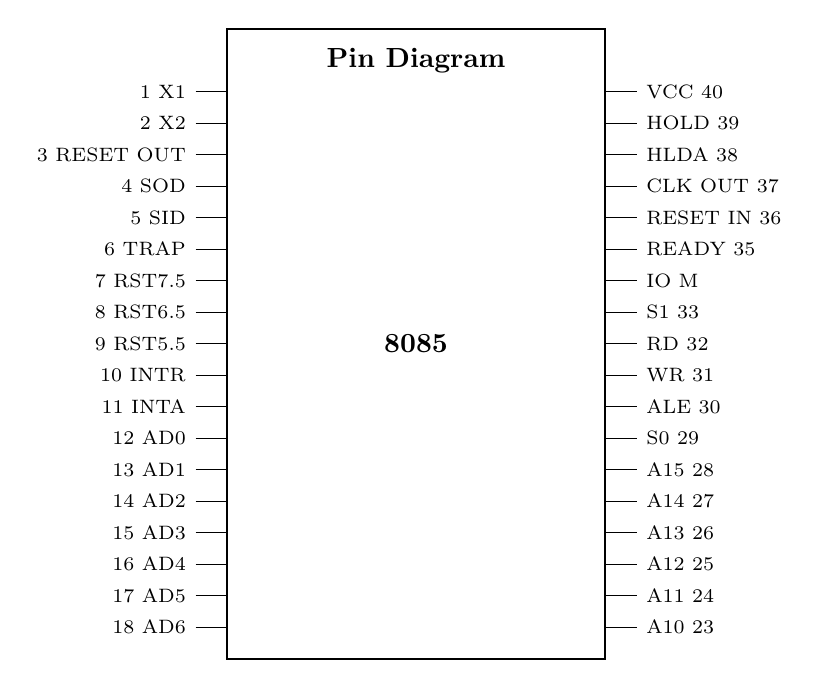
\begin{tikzpicture}[scale=0.8]
    \draw [thick] (0,0) rectangle (6,10);
    \node at (3,5) {\textbf{8085}};
    \node at (3,9.5) {\textbf{Pin Diagram}};
    
    % Left Pins
    \foreach \y/\label/\pin in {9/X1/1, 8.5/X2/2, 8/RESET OUT/3, 7.5/SOD/4, 7/SID/5, 6.5/TRAP/6, 6/RST7.5/7, 5.5/RST6.5/8, 5/RST5.5/9, 4.5/INTR/10, 4/INTA/11, 3.5/AD0/12, 3/AD1/13, 2.5/AD2/14, 2/AD3/15, 1.5/AD4/16, 1/AD5/17, 0.5/AD6/18}
        \draw (-0.5, \y) node[left] {\scriptsize \pin\ \label} -- (0, \y);
        
    % Right Pins
    \foreach \y/\label/\pin in {9/VCC/40, 8.5/HOLD/39, 8/HLDA/38, 7.5/CLK OUT/37, 7/RESET IN/36, 6.5/READY/35, 6/IO/M/34, 5.5/S1/33, 5/RD/32, 4.5/WR/31, 4/ALE/30, 3.5/S0/29, 3/A15/28, 2.5/A14/27, 2/A13/26, 1.5/A12/25, 1/A11/24, 0.5/A10/23}
        \draw (6, \y) -- (6.5, \y) node[right] {\scriptsize \label\ \pin};
\end{tikzpicture}
\captionof{figure}{8085 Pin Detail}
\end{center}

\begin{center}
\captionof{table}{Pin Description}
\begin{tabulary}{\linewidth}{|L|L|}
\hline
\textbf{Pin Group} & \textbf{Function} \\ \hline
\textbf{High Address (A8-A15)} & Carries most significant byte of address. \\ \hline
\textbf{Multiplexed (AD0-AD7)} & Carries lower address byte (T1) and Data (T2, T3). \\ \hline
\textbf{Control (RD, WR, ALE)} & READ, WRITE control and Address Latch Enable. \\ \hline
\textbf{Status (IO/M, S0, S1)} & Indicates type of machine cycle (Memory vs I/O, Read vs Write). \\ \hline
\textbf{Interrupts} & TRAP (Non-maskable), RST7.5, 6.5, 5.5, INTR. \\ \hline
\textbf{Serial I/O} & SID (Input), SOD (Output) for serial data. \\ \hline
\end{tabulary}
\end{center}
\end{solutionbox}

\questionmarks{3(a)}{3}{Draw IP SFR of 8051 and Explain function of each bit.}

\begin{solutionbox}
The Interrupt Priority (IP) register (Address B8H) determines priority levels (High/Low).

\begin{center}
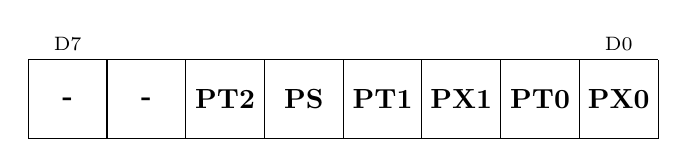
\begin{tikzpicture}
    \draw (0,0) grid (8,1);
    \foreach \x/\label in {0.5/-, 1.5/-, 2.5/PT2, 3.5/PS, 4.5/PT1, 5.5/PX1, 6.5/PT0, 7.5/PX0}
        \node at (\x, 0.5) {\textbf{\label}};
    \node [above] at (0.5, 1) {\scriptsize D7}; \node [above] at (7.5, 1) {\scriptsize D0};
\end{tikzpicture}
\captionof{figure}{IP Register}
\end{center}

\begin{itemize}
    \item \textbf{1 = High Priority}, \textbf{0 = Low Priority}.
    \item \textbf{PS}: Serial Port Priority.
    \item \textbf{PTx}: Timer x Priority.
    \item \textbf{PXx}: External Interrupt x Priority.
\end{itemize}
\end{solutionbox}

\questionmarks{3(b)}{4}{Draw and explain Timer/Counter Logic diagram for 8051.}

\begin{solutionbox}
Timers count cycles from oscillator (Timer mode) or external pin events (Counter mode).

\begin{center}
\begin{tikzpicture}[node distance=2cm]
    \node (osc) {Osc $\div$ 12};
    \node [below=1cm of osc] (pin) {Pin T0/T1};
    
    \node [gtu decision, right=2cm of osc, shape aspect=2] (mux) {C/T};
    \node [gtu block, right=1cm of mux] (tl) {TLx};
    \node [gtu block, right=0.5cm of tl] (th) {THx};
    \node [gtu state, right=1cm of th] (tf) {TFx};
    
    \draw [->] (osc) -- (mux);
    \draw [->] (pin) -| (mux);
    \draw [->] (mux) -- node[above] {Clock} (tl);
    \draw [->] (tl) -- (th);
    \draw [->] (th) -- node[above] {Overflow} (tf);
    
    \node [above=0.5cm of mux] {TRx (Run Control)};
    \draw [->] (2.5, 1.2) -- (mux);
\end{tikzpicture}
\captionof{figure}{Timer Logic Block Diagram}
\end{center}
\end{solutionbox}

\questionmarks{3(c)}{7}{Draw and Explain Block Diagram of 8051.}

\begin{solutionbox}
The 8051 is a comprehensive microcontroller with built-in memory and I/O.

\begin{center}
\begin{tikzpicture}[scale=0.9, transform shape]
    \node [gtu block, minimum height=4cm, minimum width=2cm] (cpu) {CPU};
    
    \node [gtu block, right=2cm of cpu, fill=yellow!20] (rom) {4KB\\ROM};
    \node [gtu block, below=1cm of rom, fill=green!20] (ram) {128B\\RAM};
    
    \node [gtu block, left=2cm of cpu] (timers) {Timer 0\\Timer 1};
    \node [gtu block, below=1cm of timers] (serial) {Serial Port\\(UART)};
    
    \node [gtu block, above=1cm of cpu] (interrupt) {Interrupt\\Control};
    \node [gtu block, below=2cm of cpu, minimum width=6cm] (ports) {I/O Ports P0, P1, P2, P3};
    
    % Bus
    \draw [thick, <->] (cpu) -- (rom);
    \draw [thick, <->] (cpu) -- (ram);
    \draw [thick, <->] (cpu) -- (timers);
    \draw [thick, <->] (cpu) -- (serial);
    \draw [thick, <->] (cpu) -- (ports);
    \draw [thick, <->] (cpu) -- (interrupt);
    
    \node [below=0.2cm of ports] {External Pins};
\end{tikzpicture}
\captionof{figure}{8051 Architecture}
\end{center}

\begin{itemize}
    \item \textbf{CPU}: 8-bit central processor.
    \item \textbf{Memory}: Harvard architecture. 4KB On-chip Code ROM, 128 Bytes On-chip Data RAM.
    \item \textbf{I/O Ports}: 4 ports (P0-P3), each 8-bit. Total 32 pins.
    \item \textbf{Timers}: Two 16-bit timers (T0/T1) for delays or counting.
    \item \textbf{Serial Port}: Full-duplex UART (TXD, RXD).
\end{itemize}
\end{solutionbox}

\questionmarks{3(a) OR}{3}{Draw PCON SFR of 8051 and Explain function of each bit.}

\begin{solutionbox}
PCON (Power Control) at 87H controls power modes and baud rate doubling.

\begin{center}
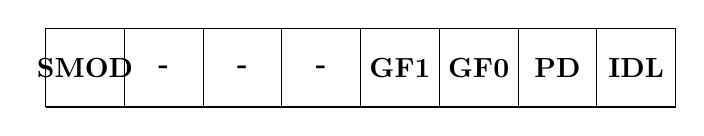
\begin{tikzpicture}
    \draw (0,0) grid (8,1);
    \foreach \x/\label in {0.5/SMOD, 1.5/-, 2.5/-, 3.5/-, 4.5/GF1, 5.5/GF0, 6.5/PD, 7.5/IDL}
        \node at (\x, 0.5) {\textbf{\label}};
\end{tikzpicture}
\captionof{figure}{PCON Register}
\end{center}

\begin{itemize}
    \item \textbf{SMOD}: Double Baud Rate. 1 = Doubles baud rate for Timer 1.
    \item \textbf{GF1/GF0}: General purpose flags.
    \item \textbf{PD}: Power Down mode. Oscillator stops.
    \item \textbf{IDL}: Idle mode. Clock to CPU stops, but Interrupts/Timers run.
\end{itemize}
\end{solutionbox}

\questionmarks{3(b) OR}{4}{In 8051 Serial communication Mode 1, For XTAL=11.0592 MHz, find TH1 value needed to have for 9600 and 4800 baud rate.}

\begin{solutionbox}
\textbf{Formula}:
\[ \text{Baud Rate} = \frac{2^{SMOD}}{32} \times \frac{XTAL}{12 \times (256 - TH1)} \]
Assuming SMOD=0 (Normal speed) and XTAL = 11.0592 MHz.

\textbf{1. For 9600 Baud:}
\[ 9600 = \frac{11059200}{32 \times 12 \times (256 - TH1)} \]
\[ 9600 = \frac{28800}{256 - TH1} \]
\[ 256 - TH1 = \frac{28800}{9600} = 3 \]
\[ TH1 = 256 - 3 = 253 = \textbf{FD H} \]

\textbf{2. For 4800 Baud:}
\[ 256 - TH1 = \frac{28800}{4800} = 6 \]
\[ TH1 = 256 - 6 = 250 = \textbf{FA H} \]
\end{solutionbox}

\questionmarks{4(a)}{3}{What are the differences in LCALL and LJMP instructions in 8051?}

\begin{solutionbox}
\begin{center}
\captionof{table}{LCALL vs LJMP}
\begin{tabulary}{\linewidth}{|L|L|L|}
\hline
\textbf{Feature} & \textbf{LCALL (Long Call)} & \textbf{LJMP (Long Jump)} \\ \hline
\textbf{Action} & Calls a subroutine. & Jumps to an address. \\ \hline
\textbf{Stack} & Pushes PC (return address) to Stack. & Does NOT affect Stack. \\ \hline
\textbf{Return} & Requires \code{RET} at end of subroutine. & No return; one-way transfer. \\ \hline
\textbf{Address} & 16-bit destination (64KB range). & 16-bit destination (64KB range). \\ \hline
\end{tabulary}
\end{center}
\end{solutionbox}

\questionmarks{4(b)}{4}{Write 8051 Assembly Language Program to generate square wave on port 1.0 using Timer0.}

\begin{solutionbox}
\begin{lstlisting}[language={[x86masm]Assembler}, caption={Square Wave Generation}]
    ORG 0000H
    LJMP MAIN

    ORG 0030H
MAIN:
    MOV TMOD, #01H      ; Timer 0, Mode 1 (16-bit)
LOOP:
    MOV TH0, #0FFH      ; Load high byte (Example value)
    MOV TL0, #000H      ; Load low byte
    SETB TR0            ; Start Timer
WAIT:
    JNB TF0, WAIT       ; Wait for Overflow Flag
    CLR TR0             ; Stop Timer
    CLR TF0             ; Clear Flag
    CPL P1.0            ; Complement P1.0 (Toggle)
    SJMP LOOP           ; Repeat
    END
\end{lstlisting}
\end{solutionbox}

\questionmarks{4(c)}{7}{Explain any three Logical and any four Data Transfer Instruction of 8051 with example.}

\begin{solutionbox}
\textbf{Logical Instructions:}
\begin{itemize}
    \item \code{ANL A, Rn}: Logical AND Register Rn with Accumulator. Result in A. \\ Ex: \code{ANL A, R2}
    \item \code{ORL A, \#data}: Logical OR immediate data with A. \\ Ex: \code{ORL A, \#30H}
    \item \code{XRL A, direct}: Logical XOR memory content with A. \\ Ex: \code{XRL A, 40H}
\end{itemize}

\textbf{Data Transfer Instructions:}
\begin{itemize}
    \item \code{MOV A, Rn}: Move content of Register to Accumulator. \\ Ex: \code{MOV A, R5}
    \item \code{MOVX A, @DPTR}: Move External RAM data pointed by DPTR to A. \\ Ex: \code{MOVX A, @DPTR}
    \item \code{PUSH direct}: Push content of memory address onto Stack. \\ Ex: \code{PUSH 0E0H} (Push A)
    \item \code{MOVC A, @A+DPTR}: Move Code Byte from ROM relative to DPTR. \\ Ex: \code{MOVC A, @A+DPTR}
\end{itemize}
\end{solutionbox}

\questionmarks{4(a) OR}{3}{Explain Instructions: (i) RRC A (ii) POP (iii) CLR PSW.7}

\begin{solutionbox}
\begin{enumerate}
    \item \textbf{RRC A}: Rotate Accumulator Right through Carry. MSB takes Carry value, Carry takes LSB.
    \item \textbf{POP direct}: Pop byte from Stack into destination address. SP is decremented.
    \item \textbf{CLR PSW.7}: Clears the Carry Flag (CY). PSW.7 corresponds to the Carry bit.
\end{enumerate}
\end{solutionbox}

\questionmarks{4(b) OR}{4}{Write 8051 Assembly Language Program to Divide data stored in location 30H by data stored in location 31H and store remainder in 40h and quotient in 41h memory location.}

\begin{solutionbox}
\begin{lstlisting}[language={[x86masm]Assembler}, caption={Division Program}]
    ORG 0000H
    MOV A, 30H      ; Dividend (Numerator)
    MOV B, 31H      ; Divisor (Denominator)
    DIV AB          ; Divide A by B
    ; Result: A = Quotient, B = Remainder
    MOV 41H, A      ; Store Quotient
    MOV 40H, B      ; Store Remainder
    END
\end{lstlisting}
\end{solutionbox}

\questionmarks{4(c) OR}{7}{List Addressing Modes of 8051 Microcontroller and Explain each with Example.}

\begin{solutionbox}
\begin{center}
\captionof{table}{8051 Addressing Modes}
\begin{tabulary}{\linewidth}{|L|L|L|}
\hline
\textbf{Mode} & \textbf{Explanation} & \textbf{Example} \\ \hline
\textbf{Immediate} & Operand is provided in the instruction itself (\#). & \code{MOV A, \#25H} \\ \hline
\textbf{Register} & Operand is in one of the registers R0-R7. & \code{MOV A, R0} \\ \hline
\textbf{Direct} & Direct memory address is specified. & \code{MOV A, 30H} \\ \hline
\textbf{Register Indirect} & Address is held in R0 or R1 (@). & \code{MOV A, @R0} \\ \hline
\textbf{Indexed} & Base address + Accumulator offset. Used for ROM lookups. & \code{MOVC A, @A+DPTR} \\ \hline
\end{tabulary}
\end{center}
\end{solutionbox}

\questionmarks{5(a)}{3}{Draw Interfacing of Relay with 8051 microcontroller.}

\begin{solutionbox}
A relay requires a driver transistor as it uses high current.

\begin{center}
\begin{circuitikz}[scale=1]
    \draw (0,0) node[anchor=east] {P1.0} to[R, l=1k$\Omega$, o-*] (2,0) -- (2.5,0)
    node[npn, anchor=B] (Q) {BC547};
    \draw (Q.E) -- (2.5,-1) node[ground]{};
    \draw (Q.C) -- (2.5,1.5);
    
    % Relay Coil
    \draw (2.5,1.5) to[L, l=Relay] (2.5,3) -- (2.5,3.5) node[vcc] {+12V};
    
    % Diode
    \draw (3.5,1.5) to[D*, l=1N4007] (3.5,3);
    \draw (2.5,1.5) -- (3.5,1.5);
    \draw (2.5,3) -- (3.5,3);
\end{circuitikz}
\captionof{figure}{Relay Interfacing}
\end{center}
\end{solutionbox}

\questionmarks{5(b)}{4}{Interface 7 Segment display with 8051 microcontroller and write a program to print "1" on it.}

\begin{solutionbox}
Assuming Common Cathode display on Port 1.

\begin{center}
\begin{circuitikz}
    \draw (0,0) node[draw, minimum height=2cm] (P1) {Port 1};
    \draw (4,0) node[draw, minimum height=2cm] (disp) {7-Seg};
    
    \foreach \y in {0.6, 0.4, 0.2, 0, -0.2, -0.4, -0.6}
        \draw [->] ($(P1.east)+(0,\y)$) -- ($(disp.west)+(0,\y)$);
        
    \node [right=0.2cm of P1] {Lines a-g, dp};
\end{circuitikz}
\captionof{figure}{7-Segment Interface}
\end{center}

\begin{lstlisting}[language={[x86masm]Assembler}, caption={Display Digit 1}]
    ; For Common Cathode, segments B, C must be 1.
    ; Pattern: dp g f e d c b a
    ; "1" -> 0 0 0 0 0 1 1 0 = 06H
    MOV P1, #06H
    END
\end{lstlisting}
\end{solutionbox}

\questionmarks{5(c)}{7}{Interface DAC 0808 with 8051 microcontroller and write a program to generate Square wave.}

\begin{solutionbox}
DAC 0808 is an 8-bit DAC. Port 2 connects to D0-D7.

\begin{center}
\begin{circuitikz}
    \draw (0,2) node[draw, minimum height=2cm] (cpu) {8051 (P2)};
    \draw (4,2) node[draw, minimum height=2cm] (dac) {DAC0808};
    \draw [->, thick] (cpu) -- node[above] {Data Bus} (dac);
    
    \draw (dac.east) -- ++(1,0) node[op amp, anchor=-] (opamp) {};
    \draw (opamp.+) -- ++(0,-0.5) node[ground] {};
    \draw (opamp.out) -- ++(0.5,0) node[right] {$V_{out}$};
    \draw (opamp.-) -- ++(0,1) -| (opamp.out); % Feedback
\end{circuitikz}
\captionof{figure}{DAC Interfacing}
\end{center}

\begin{lstlisting}[language={[x86masm]Assembler}, caption={Square Wave via DAC}]
LOOP:
    MOV P2, #00H     ; Min Voltage (0V)
    ACALL DELAY      ; Wait
    MOV P2, #0FFH    ; Max Voltage (5V)
    ACALL DELAY      ; Wait
    SJMP LOOP
DELAY:
    MOV R0, #255
DL: DJNZ R0, DL
    RET
\end{lstlisting}
\end{solutionbox}

\questionmarks{5(a) OR}{3}{Interface of Push button Switch with 8051 microcontroller.}

\begin{solutionbox}
A push button connects a pin to Ground. A pull-up resistor ensures High logic when open.

\begin{center}
\begin{circuitikz}
    \draw (0,2) node[vcc] {+5V} to[R, l=10k$\Omega$] (0,1) -- (0,-0.5) to[push button, l=Switch] (0,-1.5) node[ground]{};
    \draw (0,1) -- (2,1) node[right] {To P1.0};
\end{circuitikz}
\captionof{figure}{Switch Interface}
\end{center}
\end{solutionbox}

\questionmarks{5(b) OR}{4}{Interface DC Motor with 8051 microcontroller.}

\begin{solutionbox}
Use a Darlington Transistor (like TIP122) or MOSFET to drive the motor current.

\begin{center}
\begin{circuitikz}
    \draw (0,0) node[left] {P1.0} to[R, l=1k] (2,0) node[npn, anchor=B] (Q) {TIP122};
    \draw (Q.E) node[ground]{};
    \draw (Q.C) -- (2.77, 1.5) node[draw, circle, minimum size=0.8cm] {M} -- (2.77, 3) node[vcc]{+12V};
    \draw (4, 0.77) to[D*, l=Flyback Diode] (4, 3) -- (2.77,3);
    \draw (4, 0.77) -- (Q.C);
\end{circuitikz}
\captionof{figure}{DC Motor Driver}
\end{center}
\end{solutionbox}

\questionmarks{5(c) OR}{7}{Interface LCD with 8051 microcontroller and write a program to display "Hello".}

\begin{solutionbox}
LCD 16x2 works in 8-bit mode. Data lines to P2, Control to P3.

\begin{center}
\begin{circuitikz}
    \node [gtu block, minimum height=3cm] (lcd) {LCD 16x2};
    \node [gtu block, left=3cm of lcd, minimum height=3cm] (cpu) {8051};
    
    \draw [->, thick] (cpu.east) -- node[above] {D0-D7 (P2)} (lcd.west);
    \draw [->] ($(cpu.east)+(0,-1)$) -- node[below] {RS, RW, EN (P3)} ($(lcd.west)+(0,-1)$);
\end{circuitikz}
\end{center}

\begin{lstlisting}[language={[x86masm]Assembler}, caption={LCD "HELLO"}]
    MOV A, #38H     ; Init 2 lines, 5x7 matrix
    ACALL CMD
    MOV A, #0EH     ; Display ON, Cursor ON
    ACALL CMD
    MOV A, #'H'     ; Data H
    ACALL DAT
    MOV A, #'E'
    ACALL DAT
    ; ... (L, L, O)
    SJMP $
CMD:
    MOV P2, A
    CLR P3.0        ; RS=0 (Command)
    SETB P3.1       ; EN=1
    CLR P3.1        ; EN=0 (Latch)
    ACALL DELAY
    RET
DAT:
    MOV P2, A
    SETB P3.0       ; RS=1 (Data)
    SETB P3.1
    CLR P3.1
    ACALL DELAY
    RET
\end{lstlisting}
\end{solutionbox}

\end{document}
